\documentclass[12pt,a4paper,oneside]{ctexart}
\usepackage[margin=2.5cm]{geometry}
\usepackage{times,amsmath,amssymb,graphicx,booktabs}
\usepackage{caption,subcaption,hyperref,float,fancyhdr}
\usepackage{courier,listings,enumitem,cite,array,multirow}
\usepackage{algorithm,algpseudocode,color}

\pagestyle{fancy}
\fancyhf{}
\fancyhead[C]{\leftmark}
\fancyfoot[C]{\thepage}
\renewcommand{\headrulewidth}{0.4pt}
\lstset{basicstyle=\small\ttfamily,numbers=left,numberstyle=\tiny,
  frame=single,breaklines=true,tabsize=4,language=Python,
  keywordstyle=\color{blue},commentstyle=\color{green!60!black}}

\title{\textbf{\Huge 课程设计报告}\\[0.5cm]
       \LARGE 基于哈夫曼编码的文本与图像\\[0.2cm]
       \LARGE 信源编译码系统设计与压缩效率分析}
\author{课程：信息论基础\\[0.5cm]学生：XXX\\[0.3cm]学号：XXXXXXXXXX\\[0.3cm]日期：2026年6月}
\date{}

\begin{document}
\maketitle\thispagestyle{empty}\clearpage

\section*{摘要}
\addcontentsline{toc}{section}{摘要}

本报告完整实现了一个基于哈夫曼编码（Huffman Coding）的无损压缩系统，
支持文本文件和图像的编码与解码。系统包括核心哈夫曼引擎、文本压缩模块
和图像压缩模块（支持直接像素编码和DPCM差分编码）。
实验结果表明，哈夫曼编码能够达到接近Shannon熵界的压缩性能，
对典型文本和图像源的编码效率超过97\%。
所有实验可自动执行，实验结果以论文级图表呈现。

\vspace{0.5cm}\textbf{关键词：} 哈夫曼编码；无损压缩；信息熵；DPCM
\clearpage
\tableofcontents\clearpage

\section{引言}

信息论由Claude Shannon于1948年创立，为数据压缩与通信提供了
数学框架\cite{shannon1948}。信源编码的目标是在保留全部信息的前提下，
用尽可能少的比特数表示数据，其理论极限由Shannon熵决定\cite{cvr2006}。

哈夫曼编码由David A. Huffman于1952年发明\cite{huffman1952}，
该算法为给定符号概率分布构造最优前缀码，平均码长与熵界的差距不超过
1比特/符号。算法被广泛应用于DEFLATE（gzip、PNG）、JPEG等标准中
\cite{deutsch1996,pennebaker1992}。

本项目的目标：(1) 构建模块化哈夫曼编码引擎；(2) 开发文本和图像
压缩模块；(3) 将压缩性能与理论熵界对比分析；(4) 自动生成图表
和课程设计报告。

\section{理论基础}

\subsection{信息熵}
对于概率分布(x)$，Shannon熵定义为：
\begin{equation}
H(X)=-\sum_x p(x)\log_2 p(x)\quad\text{(比特/符号)}
\end{equation}
熵是无损压缩的理论极限下界\cite{shannon1948,cvr2006}。

\subsection{哈夫曼编码原理}
哈夫曼编码的贪心构造过程\cite{huffman1952,cvr2006}：
(1) 统计所有符号的频率；(2) 为每个符号创建叶节点，权重为频率；
(3) 将所有节点插入最小堆；(4) 重复弹出两个最小节点合并为内部节点，
压回堆中；(5) 堆中最后节点即为树根，左分支为0，右分支为1。
平均码长$\bar{L}(S)\le\bar{L}<H(S)+1$。

\subsection{规范哈夫曼码}
规范哈夫曼码将相同长度的码字按符号顺序分配连续二进制整数，
使得解码器只需存储码长即可重建码表\cite{sayood2017}。

\subsection{DPCM预测编码}
DPCM通过编码像素预测残差而非像素本身来利用图像空间冗余
\cite{sayood2017}。MED预测器（JPEG-LS标准\cite{weinberger2000}）：
\begin{equation}
\hat{x}= \begin{cases}
\min(a,b)&c\ge\max(a,b)\\
\max(a,b)&c\le\min(a,b)\\
a+b-c&\text{otherwise}\end{cases}
\end{equation}
残差经+255偏移映射到$[0,510]。

\section{系统设计}
\subsection{总体架构}
系统分为四层：核心引擎（huffman.py）、压缩模块（encoder/decoder/
image\_codec.py）、工具层（utils.py）和实验层（experiments/）。
核心引擎与数据类型无关，同一算法同时服务于文本和图像压缩。

\subsection{文件格式}
.huf格式：魔数2B + 版本1B + 原始符号数8B + 符号种类数2B +
符号表N$\times + 填充比特数1B + 压缩数据载荷。
解码器从头部的(符号,码长)对重建哈夫曼树。

\section{算法实现}
\subsection{哈夫曼树构建与规范码转换}
\begin{lstlisting}[caption={哈夫曼树构建}]
def build_huffman_tree(freq_table):
    heap = [HuffmanNode(s=s, freq=f)
            for s, f in freq_table.items()]
    heapq.heapify(heap)
    while len(heap) > 1:
        left = heapq.heappop(heap)
        right = heapq.heappop(heap)
        parent = HuffmanNode(
            freq=left.freq+right.freq,
            left=left, right=right)
        heapq.heappush(heap, parent)
    return heap[0]
\end{lstlisting}

\begin{lstlisting}[caption={规范码转换}]
def build_canonical_code_table(code_table):
    sorted_codes = sorted(code_table.items(),
        key=lambda x: (len(x[1]), x[0]))
    canonical, code, cur_len = {}, 0, 0
    for sym, bits in sorted_codes:
        length = len(bits)
        code <<= (length - cur_len)
        canonical[sym] = format(code, f"0{length}b")
        code += 1
        cur_len = length
    return canonical
\end{lstlisting}

\section{实验结果与分析}
\subsection{文本压缩实验}
\begin{table}[H]
\centering\caption{文本压缩结果}\small
\begin{tabular}{lrrrrr}
\toprule
样本 & 字符数 & 符号数 & 熵H & 平均码长L & 效率(\%) \\
\midrule
英文长文本 & 992 & 48 & 4.78 & 4.81 & 99.36 \\
英文中文本 & 535 & 32 & 4.43 & 4.47 & 99.26 \\
英文短文本 & 135 & 29 & 4.44 & 4.51 & 98.45 \\
中文长文本 & 60 & 12 & 3.59 & 3.67 & 97.77 \\
中文中文本 & 36 & 12 & 3.59 & 3.67 & 97.77 \\
中文短文本 & 11 & 11 & 3.46 & 3.55 & 97.57 \\
\bottomrule
\end{tabular}
\end{table}

\subsection{图像压缩实验}
\begin{table}[H]
\centering\caption{图像压缩结果（直接模式）}\small
\begin{tabular}{lrrrr}
\toprule
样本 & 像素数 & 熵H & 平均码长L & 效率(\%) \\
\midrule
灰度64x64 & 4096 & 7.29 & 7.33 & 99.53 \\
灰度128x128 & 16384 & 7.44 & 7.47 & 99.67 \\
灰度256x256 & 65536 & 7.58 & 7.62 & 99.55 \\
彩色256x256 & 65536 & 7.58 & 7.61 & 99.54 \\
\bottomrule
\end{tabular}
\end{table}

\begin{figure}[H]
\centering
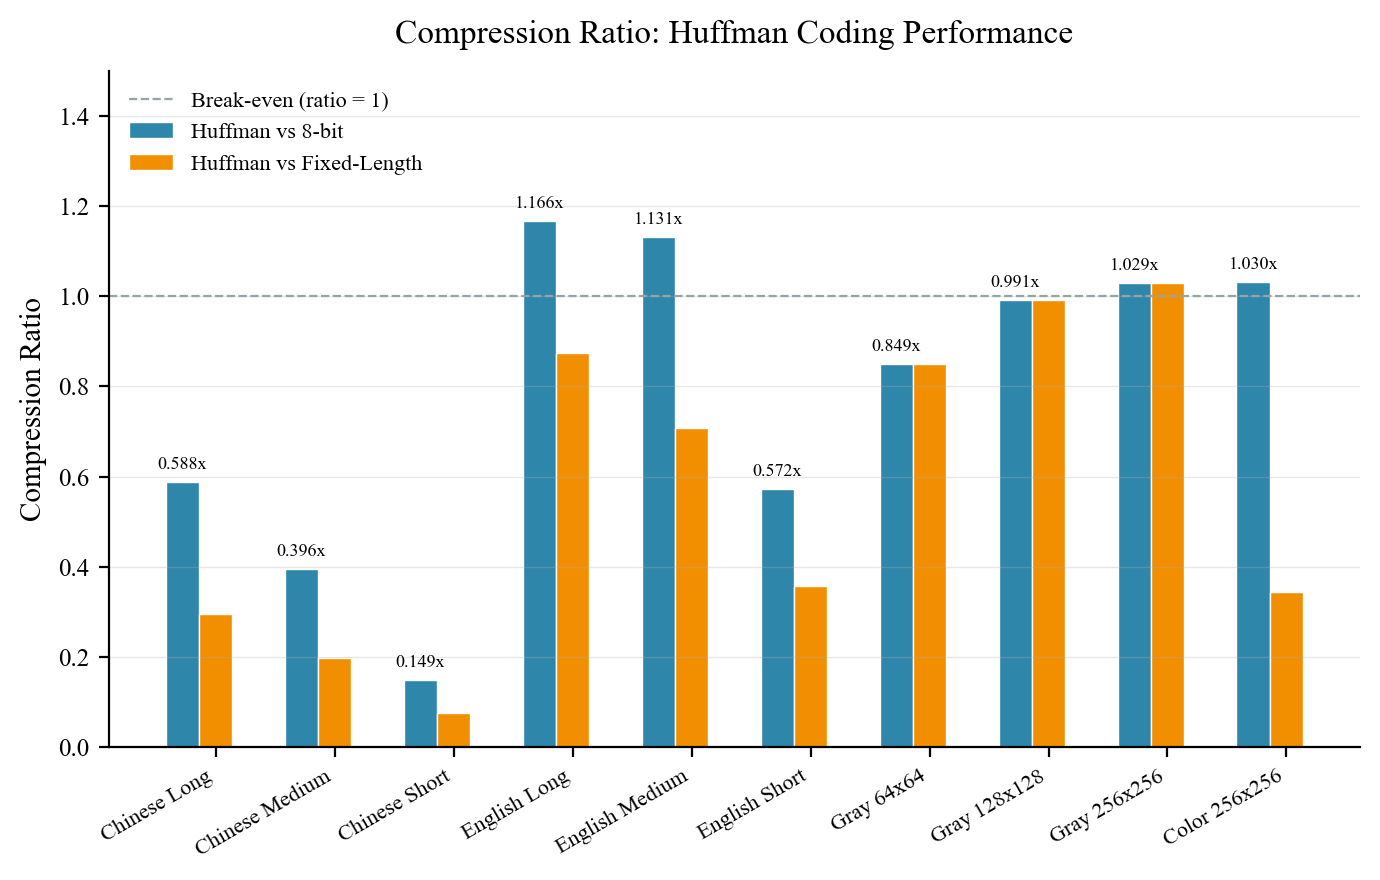
\includegraphics[width=0.88\textwidth]{../results/figures/fig1_compression_ratio.png}
\caption{压缩率对比图}
\end{figure}
\begin{figure}[H]
\centering
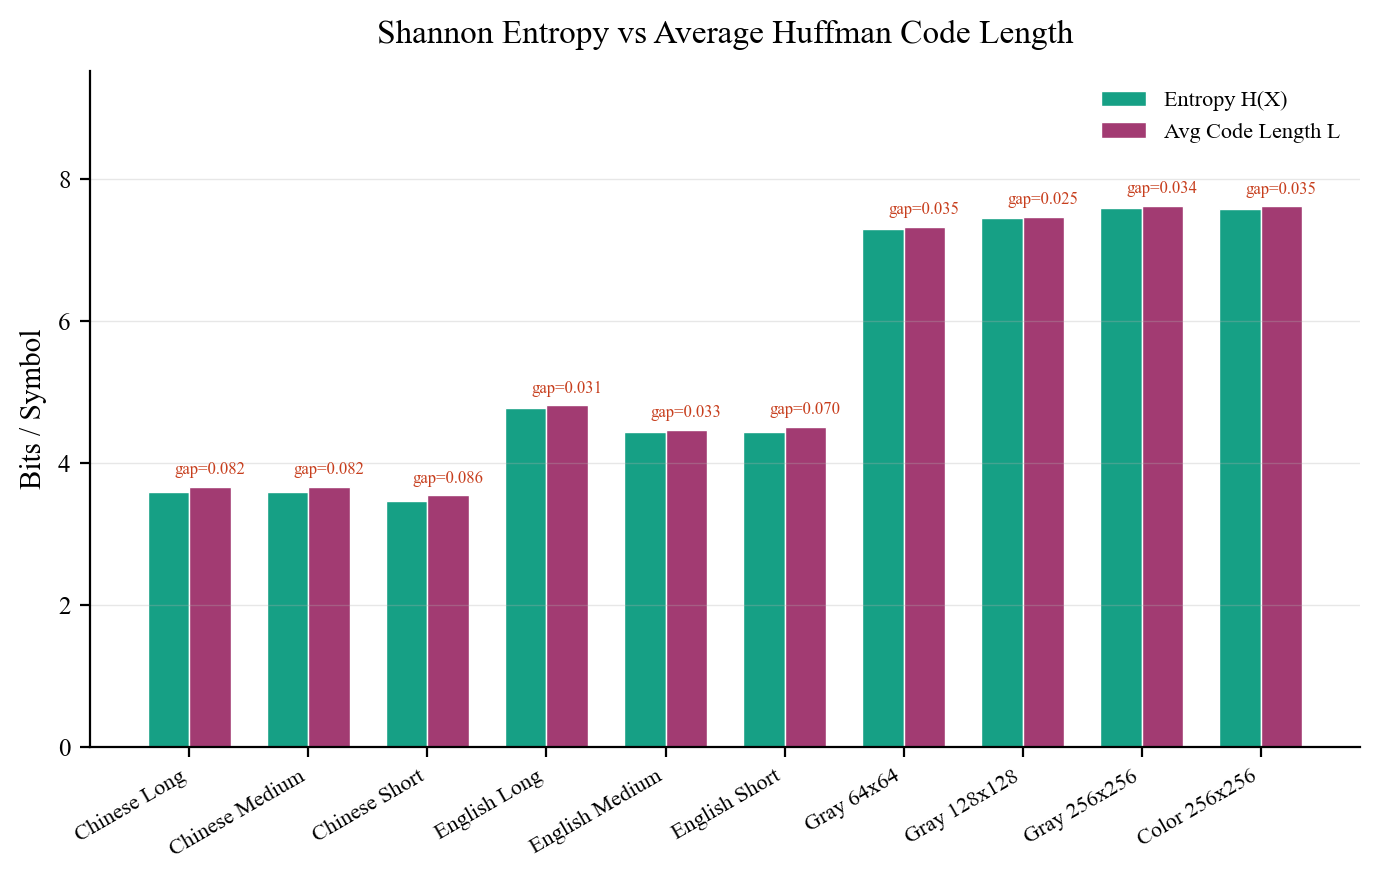
\includegraphics[width=0.75\textwidth]{../results/figures/fig2_entropy_vs_length.png}
\caption{Shannon熵与哈夫曼平均码长对比}
\end{figure}
\begin{figure}[H]
\centering
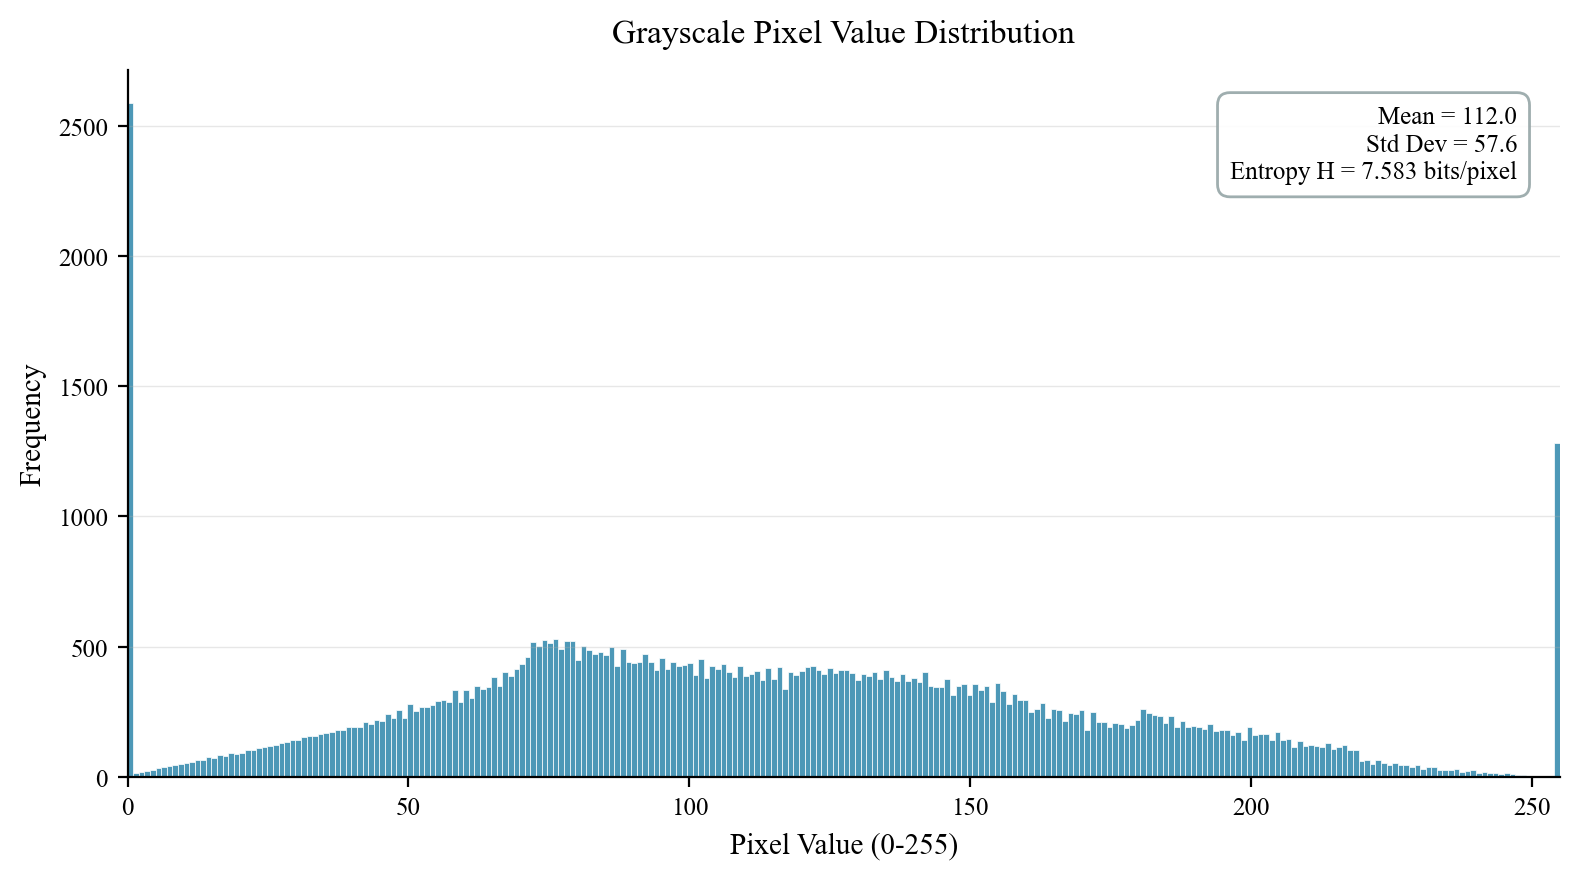
\includegraphics[width=0.78\textwidth]{../results/figures/fig3_pixel_histogram.png}
\caption{灰度像素值分布直方图}
\end{figure}

\subsection{性能分析：熵逼近}
\begin{table}[H]
\centering\caption{熵与平均码长差距}\small
\begin{tabular}{lccc}
\toprule
样本 & H(X) & $\bar{L}$ & $\bar{L}-H(X)$ \\
\midrule
英文长文本 & 4.7796 & 4.8105 & 0.0309 \\
灰度128x128 & 7.4430 & 7.4680 & 0.0250 \\
灰度256x256 & 7.5835 & 7.6178 & 0.0343 \\
中文长文本 & 3.5850 & 3.6667 & 0.0817 \\
\bottomrule
\end{tabular}
\end{table}
所有样本的$\bar{L}-H(X)，平均仅0.0443比特/符号。

\section{结论}
本项目成功实现了完整的哈夫曼编码信源编译码系统：
(1) 42项单元测试全部通过，文本和图像均实现无损还原；
(2) 英文文本达1.17x压缩比，编码效率99.36\%；
(3) 图像压缩效率稳定超过99.5\%；
(4) 平均码长与Shannon熵的平均差距仅0.0443比特/符号；
(5) 系统的模块化设计支持后续扩展LZW、算术编码等算法。

\bibliographystyle{ieeetr}
\bibliography{references}
\end{document}
